So far, all we've done is watch things blink. Now, it's time to take control.

\GOALS
Connect a button to the Arduino and use it to turn an LED on and off.

\CODE
\lstinputlisting[caption=Using a button to toggle an LED on and off.,label=code:button-toggle-led]{code/button-toggle-led.occ}

Before this code will do anything interesting, we'll have to build another circuit.

\section{The Circuit}
For this circuit, we'll add a button to the Arduino that turns the built-in LED on and off. To do this, we'll need to see how to attach a button to the Arduino.

You will need:
\begin{enumerate}
	\item Your Arduino
	\item A button
	\item Some jumper wire
	\item A 10k\ohm resistor
\end{enumerate}

A picture of what you're going to build (and the circuit diagram) can be found in Figure~\vref{diagram:button-circuit}.

\begin{figure}[h]
  \begin{center}
    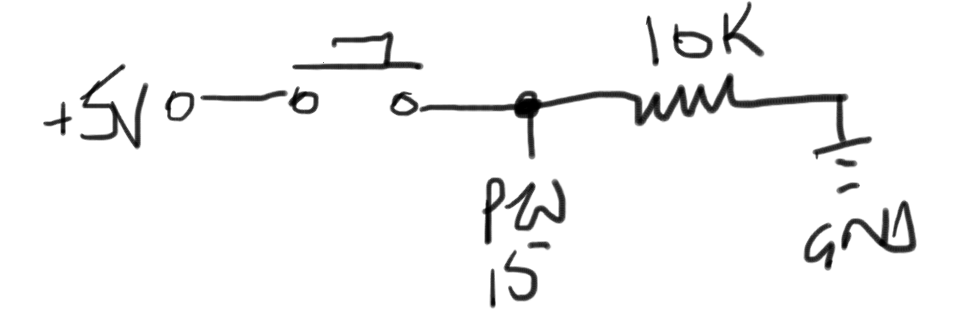
\includegraphics[width=0.6\linewidth]{images/ch4-button-circuit}
    \caption{Connecting a button to the Arduino.}
    \label{diagram:ch4-button-circuit}
  \end{center}
\end{figure}

To build the circuit, place the button on your breadboard, and run a jumper from the {\code +5V} pin on the Arduino to the same column as one corner of the button. Then, from the opposite corner, connect a 10k\ohm resistor (Brown Black Orange Gold). Connect the other end of the resistor to the {\code GND} pin on the Arduino with a jumper wire. If you forget the resistor, or use the wrong one, you could damage your Arduino---the resistor makes sure that too much current cannot flow from the voltage source to ground and damage our Arduino in the next step.

You see, the circuit we have built doesn't yet connect to any pins that we can detect changes on. The {\code +5V} pin is just a power outlet. Plugging into {\code +5V} is like plugging something into an electrical socket in your house. The {\code GND} pin is the other end of the circuit; in most homes, there is actually a copper rod that goes from the electrical junction box into the actual ground. To prevent too much current from flowing through this circuit, we use a resistor 10K\ohm resistor to bring the current down to levels that the Arduino can safely measure.

So, to complete your circuit, connect the ``high side'' of the resistor to pin 2 on the Arduino. The ``high side'' is the side that is closer to the {\code +5V} pin in the circuit. (The ``high side'' of the resistor is also the ``low side'' of the button, if that helps at all.)

\subsection{Test it!}
If you've assembled your circuit correctly, you should be able to run the program from this chapter and use the button to turn the built-in LED on and off!

\PATTERNS
% We? You? Need to get this straight throughout the text. Make a decision. Are we talking with them, or two them, or do we avoid this kind of language all together?
In the previous chapter, we saw how to run two processes in \PARallel. Specifically, we were able to blink two LEDs at the same time, and (if we wanted), both could blink at different rates. However, the rate of one LED did not, in any way, affect the blink rate of the other LED.

In this program, the button is clearly turning the LED on and off. To do this, we've built our first {\em process network}. That is, we have more than one process that is executing in parallel, and one is communicating information to the other.

%Perhaps intro some diagrams in chapter 3, since it is so light-weight at the moment?
\subsection{A two-process network}
\plumbing is all about connecting one parallel process up to another and communicating information between those processes. This turns out to be a highly visual notion, so we like to draw pictures of our process networks whenever possible.
 
\begin{figure}[h]
  \begin{center}
    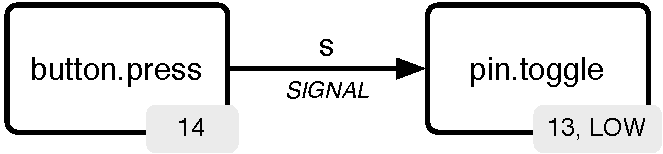
\includegraphics[width=0.8\linewidth]{images/ch4-button-toggle-led}
    \caption{A communicating two-process network.}
    \label{diagram:ch4-button-toggle-led}
  \end{center}
\end{figure}

This diagram tells us a great deal about the \plumbing program that we're writing. We'll repeat that here, so you don't have to flip pages:

\lstinputlisting[caption=The code and diagram are related.]{code/button-toggle-led.occ}

\begin{itemize}
	\item Each box in the diagram represents a process. Because there are two boxes in the diagram, we can expect to find a \PAR in our code with two processes indented underneath it. 
	\item The two processes are connected by a single \CHANnel. A channel carries information in one direction only, from one process to another. In this diagram, the channel's name is {\code s}.
	\item Each process takes some other parameters; in this case, the process called \bp takes a pin number; the process \tp takes both a pin number as well as whether it should start out \LOW or \HIGH.
\end{itemize}

Process network diagrams are a good way to think about \plumbing programs. We will see many more pictures of process networks, and will see how they are converted into code time and again. This is your first introduction, and we'll spiral deeper into these ideas in the coming chapters.

\subsection{The channel}
We need a \CHANnel to share information from one process to another in a \plumbing program. Actually, it is the {\em only} way to get information from one process to another. When you want to use a channel, you first have to {\strong declare} that channel in your code. The pattern for declaring a channel can be found in Figure~\vref{diagram:pattern-channel-decl}.

\begin{figure}[h]
  \begin{center}
    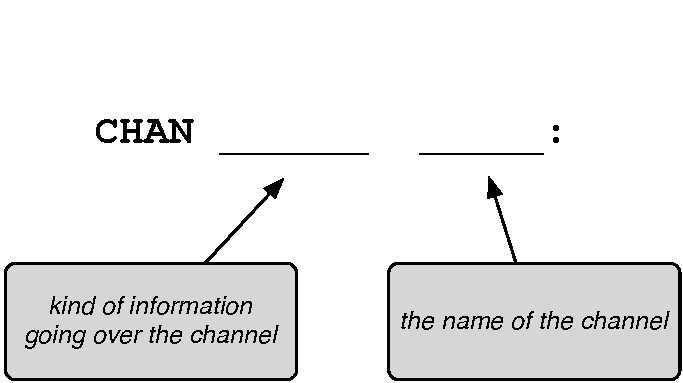
\includegraphics[width=0.6\linewidth]{images/ch4-pattern-channel-decl}
    \caption{How to declare a channel.}
    \label{diagram:ch4-pattern-channel-decl}
  \end{center}
\end{figure}

The first blank contains the {\em kind} of information that is going over the channel. If you prefer, you can think of each channel as having a particular shape, and only information that matches that shape can travel through the channel. In this chapter's code, we are sending a \SIGNALV over the channel---think of it as a sonar ping that a submarine might emit.

The second blank is the {\em name} of the channel. As the programmer, you get to choose the channel name. When we are naming channels within a \PROC, we will typically give them single-letter names. So, this channel is named {\code s}. 

The last thing to note about declaring a channel is that it typically comes before a \PAR. When we do this, every process indented under the \PARallel block then has access to the channel. This does not mean that every process in the block may {\em use} the channel. This is because every channel has two ends: a sending end, and a receiving end.

\subsubsection{How communication works}

\begin{figure}[h]
  \begin{center}
    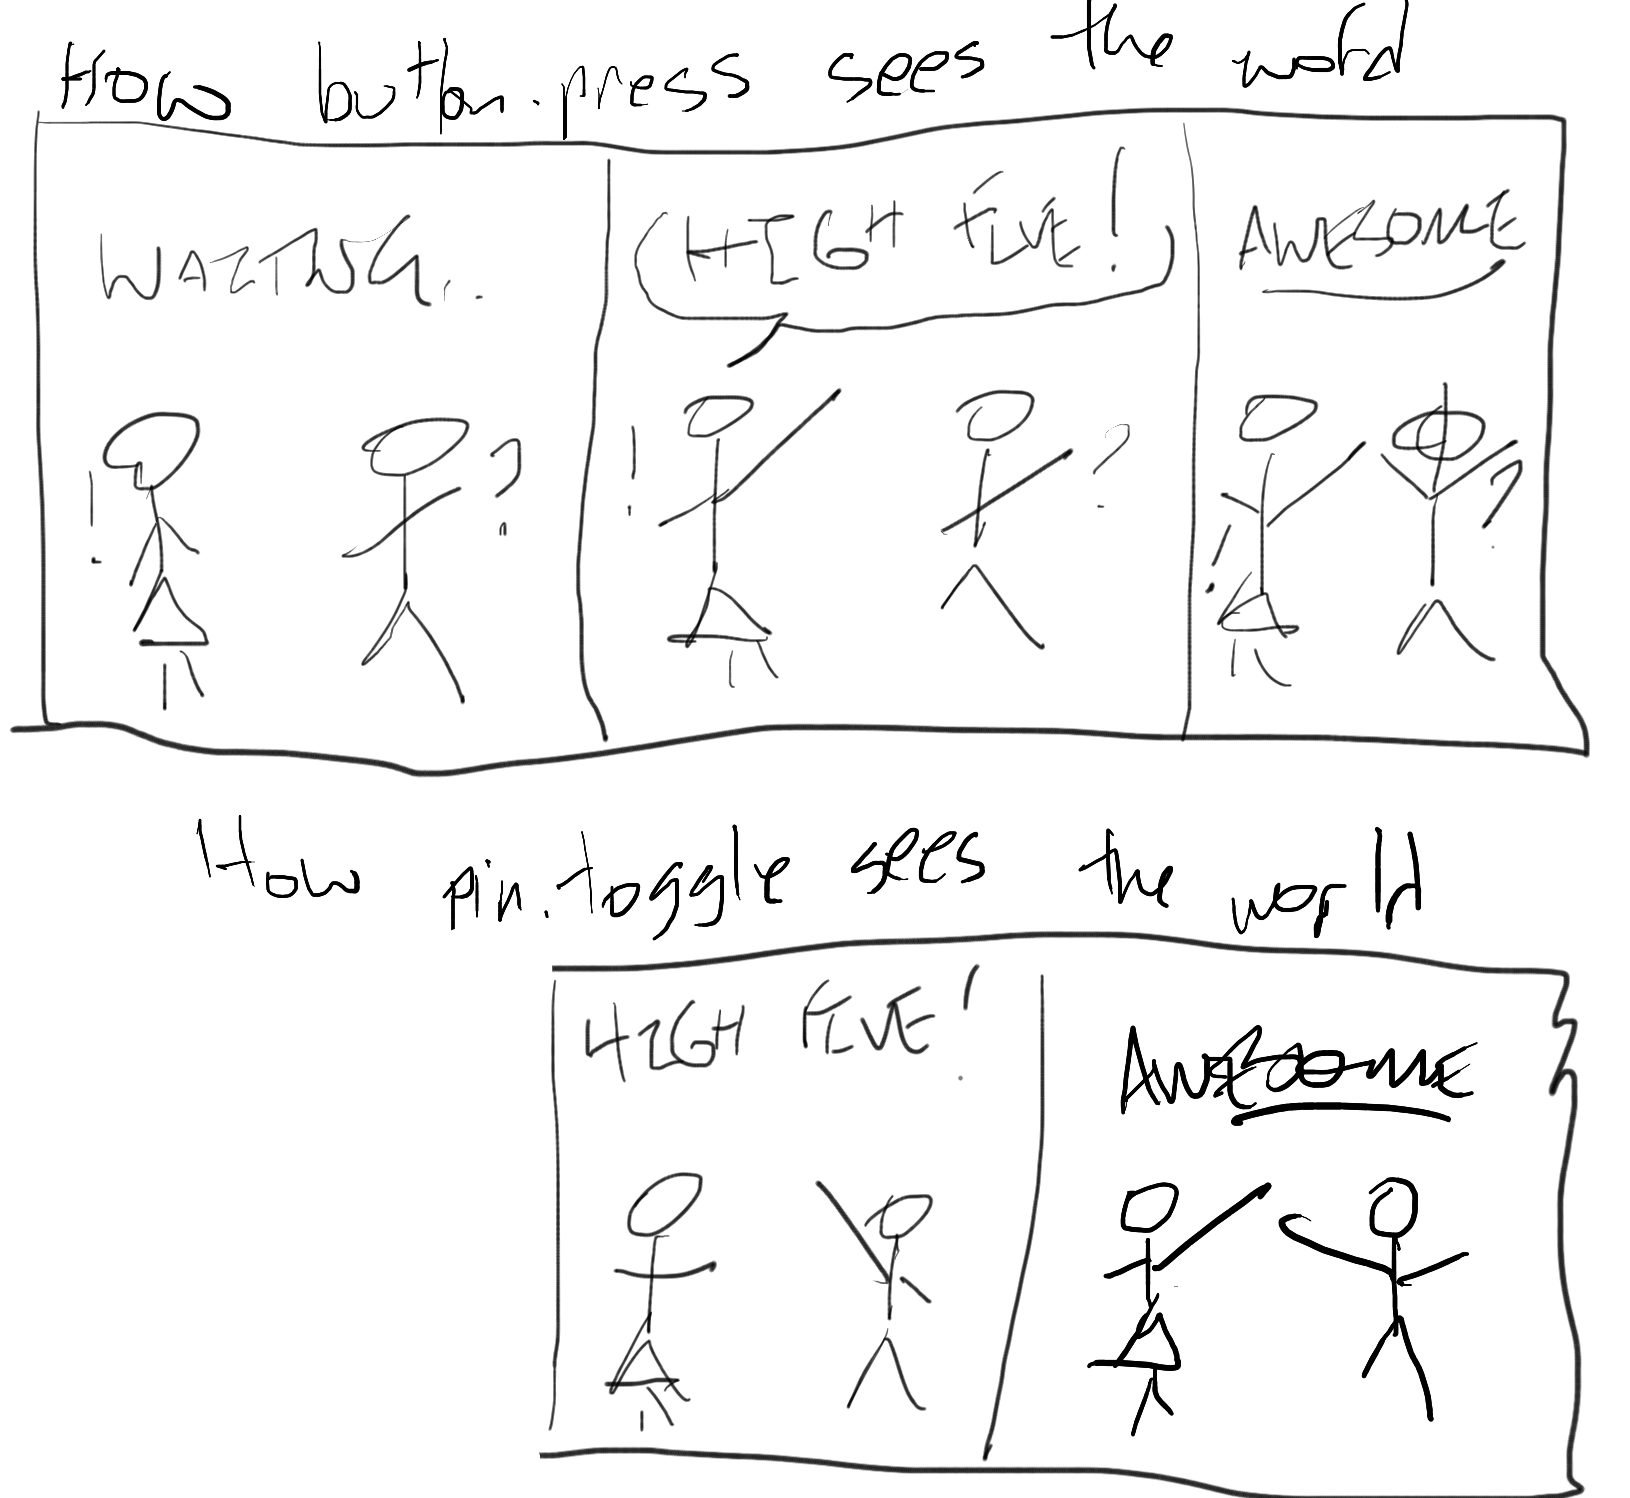
\includegraphics[width=0.8\linewidth]{images/ch4-high-five-channel-comms}
    \caption{Channel communication is like a high-five.}
    \label{diagram:ch4-high-five-channel-comms}
  \end{center}
\end{figure}

Channel communication is like giving your friend a high-five (Figure~\vref{diagram:high-five-channel-comms}).


The process \bp sits around waiting for you to press the button. When you do, it says ``high five!'' over the channel {\code s}. It then waits until \tp gets around to completing the high five, at which point the \SIGNALV has been passed from one process to another. (This, of course, is awesome.)

From the point of view of the \tp process, it says ``high five?,'' and hopes that \bp won't leave it hanging. However, \tp will wait forever, if necessary, for a \SIGNALV from \bp. When you get around to pushing the button on the Arduino, \bp completes the high five with \tp, and your LED turns on or off.


\subsubsection{The sending end of a channel}
The \bp process holds the sending end of the channel. That is because we want a \SIGNALV sent to the \tp process whenever the button is pressed. To make it clear that \bp holds the sending end of the channel, we provide the channel as a parameter to the process, but put an exclamation point after the channel name. Think of it as shouting: the \bp process will be shouting! some information to the process at the other end of the channel.

\subsubsection{The receiving end of a channel}
The \tp process is listening for a signal. It will wait all day if necessary, and until it hears a message on the channel, it won't do anything. That is why the parameter {\code s?} has a question mark: it means that \tp is saying ``what? huh?,''waiting for \bp to send it a message.

\subsection{A few quick words}
Just a few quick words about the other new things in this chapter's code.

\subsubsection{A quick word about \LOW and \HIGH}
We thought we should mention this briefly: there is a reason we do not say {\code ON} and {\code OFF} in our code. You see, LEDs turn on at a specific voltage, but it isn't 5V. It is actually somewhere inbetween 0V and 5V, and it is a little different for every LED. For that reason, we say that we drive a pin \LOW when we take it down near 0V, and we drive a pin \HIGH when we take it up near 5V. So, to turn an LED on, we drive its pin \HIGH; to turn it off, we drive that pin \LOW. Why people call it ``driving a pin'' is another thing entirely.

\subsubsection{A quick word about the dot in \bp}
The {\code .} in \bp doesn't mean anything. It is how, in \plumbing programs, we insert a space into the name of a process. You see, you can't use spaces, so we use a dot. (If you're familiar with Java, please forget everything you have ever learned about the dot. It doesn't apply here.)

\subsubsection{Channel ends as parameters}
Up until now, you have only seen numbers as parameters. Channel ends can be parameters, too. Otherwise, how would one process talk to another?

\subsubsection{\LOW and \HIGH as parameters}
\LOW and \HIGH are what we call {\em constants}. They get converted into numbers when you send your program to the Arduino. So, instead of putting ``magic numbers'' in your code (which you might forget the meaning of), you can use \LOW and \HIGH anywhere that we might talk about whether we should drive a pin to full voltage or zero voltage.

\BREAKAGE
There are lots of ways to break the code in this chapter, as usual.

\begin{description}		
	\item[Forget the colon]\ \\
	At the end of the \CHANnel declaration, remove the colon. What happens? This is a common error made by many.
	\item[Indent the PAR]\ \\
	What happens if you indent the \PAR two spaces under the \CHAN? We suspect this makes \plumbing unhappy. This is rather common as errors go as well.

	\item[Swap {\code !} and {\code ?}]\ \\
	Try switching the location of the {\code !} and {\code ?}. 
	
	\item[Leave out the {\code !} and {\code ?}]\ \\
	Try it. As it happens, this isn't an error. Perhaps it should be?
	
	\item[Forget the \SIGNALT]\ \\
	When we write \CHAN \ \SIGNALT \ {\code s}, we are telling \plumbing that the channel carries information of the type \SIGNALT over the channel {\code s} and nothing else. What happens if you delete the word \SIGNALT?
	
	\item[Forget the {\code s}]\ \\
	When we write \CHAN \ \SIGNALT \ {\code s}, we are telling \plumbing that the channel is named {\code s}. What happens if you remove the letter {\code s}?
		
\end{description}


	
	
